\section{Ejercicio 1}

\subsection{Interpretación del enunciado}
\par{En este ejercicio se habla de un señor llamado Pascual, quien trabaja en un centro de distribución del correo y se encarga de ubicar los paquetes que llegan al centro, en camiones para ser entregados. Cada uno de estos paquetes tiene un peso determinado, por lo tanto un cami\'on solo puede ser cargado con un conjunto de paquetes tales que la suma de sus pesos no exceda el l\'imite de peso del cami\'on, el cual es el mismo para todos los camiones. Pascual tiene una forma particular de hacer su trabajo, nos dicen que intenta ubicar cada paquete que llega en el camión menos cargado de los que est\'an en uso y si no llegara a entrar, usa un nuevo camión de los infinitos que tiene a su disposicion para guardarlo.}
\par{Como se trata de pesos, todos estos valores son positivos y cada paquete entra en un camión, así que el peor caso (con respecto a recursos materiales) sería necesitar un camión para cada paquete.}
\par{El objetivo es escribir un algoritmo que permita, conociendo el l\'imite de peso de los camiones y los pesos de cada paquete, saber cu\'antos camiones necesitar\'a Pascual para organizar todos los paquetes y que tan cargado estar\'a cada uno, seg\'un su metodolog\'ia de distribuci\'on. Se pide que la complejidad del algoritmo sea estrictamente menor a O($n$^{2})$ siendo $n$ la cantidad de paquetes$.}


\subsection{Resolución}
\par{El m\'etodo inmediato para resolver un problema de predicci\'on es simular la situaci\'on. Se ha desarrollado un algoritmo que reproduce el m\'etodo de Pascual y, una vez finalizado, obtiene los camiones necesarios y sus respectivas cargas (en peso). A continuaci\'on se muestra el pseudo-código de la solución. La entrada se supone ya leída y guardada en la variable $capacidadMaxima$ (la capacidad de cada cami\'on) y en una lista de paquetes (el peso de cada paquete) ordenada según su llegada. Además vamos a usar una cola de prioridad para almacenar los camiones, la cual se va a agrandar tanto como necesitemos.}

\begin{algorithm}[H]
	\caption{Llenado de camiones}
	\begin{algorithmic}
	\KwData{int $capacidadMaxima$, lista(Paquete) $paquetes$, cola\_prioridad(Camión) $camiones$}
	\ForEach{Paquete $p$ \in paquetes } {
		\eIf{peso($camionMenosCargado$) + peso(p) \leq $capacidadMaxima$ } {
			le sumo peso(p) a peso($camionMenosCargado$)\;
		}{
			agrego otro camión con peso p a $camiones$\;
		}
	}
	\end{algorithmic}
\end{algorithm}

\par{Se asume que la instrucci\'on $ForEach$ (l\'inea 1) recorre la lista en orden. Lo que se hace es tomar cada paquete de la lista y ubicarlo en un cami\'on. Tal como lo har\'ia Pascual, si el paquete entra en el cami\'on menos cargado (l\'inea 2) se lo ubica en \'el. Si no, se lo ubica en un cami\'on vac\'io (l\'inea 5). $camionMenosCargado$ representa al cami\'on cuya carga actual es la menor de entre los camiones utilizados (que ya tienen al menos un paquete). Es el menor elemento de $camiones$ (el elemento con mayor prioridad de la cola) y debe ser actualizado tras cada iteraci\'on, ya que se actualiza la carga del cami\'on menos cargado (por lo que podr\'ia dejar de ser el menos cargado) o la de un cami\'on nuevo (el cual podr\'ia pasar a ser el nuevo menos cargado).}

\subsection{Complejidad}
\par{Como usamos una cola de prioridad \footnote{Introduction to Algorithms, Thomas H. Cormen. Pagina 163 } implementada con un heap, obtener el cami\'on menos cargado consiste en tomar el m\'inimo del heap en tiempo constante. Si se modifica su valor, este debe ser extra\'ido del heap y reinsertado con otro valor (su nuevo peso). Ambas operaciones se realizan en tiempo logar\'itmico en el tama\~no del heap. Si en lugar de modificar el m\'inimo, se agrega un nuevo elemento, tambi\'en se debe realizar una inserci\'on en tiempo logar\'itimico al heap. El tama\~no del heap es la cantidad de camiones utilizados, pero est\'a acotada por la cantidad de paquetes, ya que no tendr\'ia sentido usar m\'as camiones que paquetes. Finalmente, la complejidad del algoritmo es O($n$ log($n$)) con $n$ la cantidad de paquetes, ya que se realizan $n$ iteraciones y en cada una se realizan a lo sumo dos operaciones logar\'itmicas en la cantidad de paquetes.}

\subsection{Implementaci\'on}
\par{El conjunto de camiones es implementado con la cola de prioridad\footnote{http://en.cppreference.com/w/cpp/container/priority\_queue} de la librer\'ia est\'andar de C++. En lugar de guardar la carga de cada cami\'on, se guarda la capacidad libre (es decir la capacidad m\'axima menos la suma de los pesos de los paquetes), por lo que el primer elemento no es el de menor valor sino el de mayor. Tanto la estructura como las complejidades son equivalentes. Este heap nos permite acceder en tiempo constante al primer elemento del conjunto y agregar y sacar elementos en O(log(tamaño del heap)). La operación de sumar el peso de un paquete en realidad es sacar un elemento y agregar otro con el peso sumado, lo cual es de complejidad logarítmica seg\'un la documentaci\'on de la librer\'ia.}

\subsection{Demostraci\'on de Correctitud}
\par{
En esta secci\'on demostraremos por el absurdo que la distribuci\'on de los paquetes de nuestro algoritmo es igual a la de Pascual.



Supongamos que la distribuci\'on de los paquetes de nuestro algoritmo no es la misma a la de Pascual.
Entonces deber\'ia existir un paquete que no fue asignado por nuestro algoritmo al mismo cami\'on al que lo asign\'o Pascual.
Dado que recorremos los paquetes en el mismo orden que lo hace Pascual (el orden de llegada), sea $P_i$ el primer paquete que no se asigna de la misma manera.
Entonces todos los paquetes anteriores (de $P_1$ a $P_{i-1}$) fueron asignados al mismo camión. Por lo tanto hasta ese momento la carga de cada cami\'on es igual para ambos m\'etodos.
Existen dos casos posibles:
\begin{enumerate}
	\item El paquete $P_i$ entra en el cami\'on menos cargado (el peso de $P_i$ es menor o igual a la capacidad libre del cami\'on).
	\item El paquete $P_i$ no entra en el cami\'on menos cargado (el peso de $P_i$ es mayor a la capacidad libre del cami\'on).
\end{enumerate}

En el primer caso Pascual lo ubicar\'ia en el camion menos cargado. Como \\


peso($P_i$) \leq capacidadLibre($CMC$) \Rightarrow peso($CMC$) + peso($P_i$) \leq $capacidadMaxima$  \\

entonces nuestro algoritmo entra por la primera guarda y tambi\'en ubica el paquete $P_i$ en el camion menos cargado(CMC).

En el otro caso Pascual lo ubicar\'ia en un nuevo cami\'on vac\'io. Como no se cumple la condici\'on enunciada previamente, el algoritmo entra por la sentencia correspondiente al $else$, lo que significa que agrega un cami\'on vac\'io y ubica el paquete en el nuevo cami\'on.
Como en ambos casos el algoritmo determin\'o ubicar el paquete en el mismo cami\'on que lo har\'ia Pascual, el paquete $P_i$ se lo asigna de la misma manera, lo cual genera un absurdo con la suposici\'on de que el paquete $P_i$ se asigna de forma distinta.
}

\newpage
\subsection{Testing}
\textbf{Correctitud}\\

Los tests expuestos a continuación fueron diseñados con el fin de verificar diferentes casos particulares que pudimos identificar. Para cada test vamos a exponer la entrada, la salida y, en caso de que sea necesario, una justificaci\'on de la correctitud de la soluci\'on.\\

\noindent\textbf{Test$\#$1}\\
\textbf{Caracterización:} Varios paquetes todos con pesos de modo tal que todos vayan en camiones distintos.\\
\textbf{Input:} \textfff{100 4 90 90 90 90}\\
\textbf{Output:} \textfff{4 90 90 90 90}\\
\textbf{Status:} OK. Los 4 paquetes van a distintos camiones.\\

\noindent\textbf{Test$\#$2}\\
\textbf{Caracterización:} Varios paquetes al mismo camión.\\
\textbf{Input:} \textfff{100 4 10 10 10 10}\\
\textbf{Output:} \textfff{1 40}\\
\textbf{Status:} OK. Todos van al primer camión.\\

\noindent\textbf{Test$\#$3}\\
\textbf{Caracterización:} Todos en disitintos camiones, salvo el \'ultimo que entra en el primer camión que se lleno.\\
\textbf{Input:} \textfff{100 5 80 30 30 30 15}\\
\textbf{Output:} \textfff{2 95 90}\\
\textbf{Status:} OK. No se "olvida" de los camiones que dejan de ser los menos cargados y luego vuelven a serlo.\\

\noindent\textbf{Test$\#$4}\\
\textbf{Caracterización:} Cambiando de camiones m\'as liberados (dos camiones).\\
\textbf{Input:} \textfff{100 5 55 60 15 15 15}\\
\textbf{Output:} \textfff{2 85 75}\\
\textbf{Status:} OK. \\

\noindent\textbf{Test$\#$5}\\
\textbf{Caracterización:} Respeta el orden en el cual los camiones fueron requeridos.\\
\textbf{Input:} \textfff{7 4 7 2 6 3}\\
\textbf{Output:} \textfff{3 7 5 6}\\
\textbf{Status:} OK. \\

\newpage


\textbf{Performance}
Necesitamos un gr\'afico que muestre como se comporta nuestro algoritmo a medida que la cantidad de paquetes incrementa. Para lograr esto nos hicimos un generador de casos al azar donde lo \'unico que buscamos fue poder generar muchas instancias r\'apidamente\footnote{Las mediciones de tiempos de las instancias se encuentran en codigo/ej1/tests/test.out}. Ejecutamos nuestro algoritmo midiendo los tiempos para cada corrida repitiendo varias veces cada tamaño de entrada medido y logramos el siguiente gr\'afico. 



\begin{figure}[H]
\centering
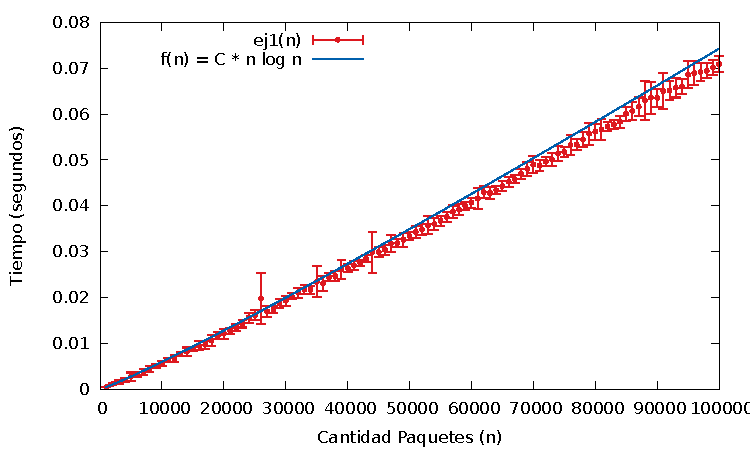
\includegraphics{imgs/ej1-graphic.pdf}
\caption{Test Performance: Tiempo(s) vs Cantidad de Paquetes.}
\end{figure}

La función f = C * n log(n), donde C = $\frac{1}{15500000}$. Se midió el tiempo con n desde 1 hasta 100000 con saltos de a 1000 (con 30 mediciones por cada n).\\
Hay que notar que las franjas para cada tamaño de entrada muestran el desvío estandar de todos los valores conseguidos para ese tamaño, esto nos pareci\'o mucho m\'as significativo que simplemente mostrar el maximo y el m\'inimo, ya que estos valores pueden variar mucho por otros procesos que pueda estar ejecutando la computadora a la vez, a pesar de que el ruido que tengamos en las mediciones no sea gaussiano.


